\section{Chart::Direction}
\herv{Name:} Chart::Direction\\ \\
\herv{File:} Direction.pm\\ \\
\herv{Requires:}Chart::Base, GD, Carp, FileHandle\\ \\
\herv{Description:} \fett{Direction} is a \fett{subclass} of Chart::Base.\\
The class Direction creates a diagram for polar coordinates.\\
Direction plots data, which is specified by angle (eg. wind direction) and value (eg. wind strength). The first dataset to add is a set of angles in degrees. The second set is a set of values. Following sets have no influence.\\ 
In the default case, direction will draw a point chart. You can also get a lines chart by turning the option 'point' to 'false' and the option 'line' to 'true'. If you want a linespoint chart, then 'point' and 'line' has to be 'true'. Additionally chart plots arrows from the center to the point or to the end of the line, if the option 'arrow' is set to 'true'.\\
\\
\herv{Example:}
\begin{figure}[h]
	\begin{center}
		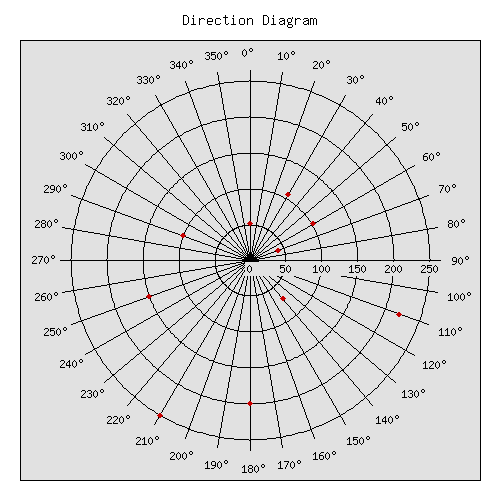
\includegraphics[width = 8cm, height =8cm]{ort.png}
	\end{center}
	\caption{Direction chart}
	\label{fig:direction}
\end{figure}
\begin{verbatim}
use Chart::Direction;
$g = Chart::Direction->new(500,500);

$g->add_dataset(0, 180, 290, 70, 60, 250, 210, 30, 110, 140 );
$g->add_dataset(50, 200, 100, 40, 100, 150, 250, 105, 220, 70);

%hash = ( 'title' => 'Direction Diagram',
          'legend' => 'none',
          'precision' => 0,
          'angle_interval' => 10,
          'pt_size' => 10);
      
$g->set(%hash);
$g->png("Grafiken/ort.png");
\end{verbatim}
\herv{Constructor:} An instance of a direction chart object can be created with the constructor new():\\
\fett{\$obj = Chart::Direction->new();}\\
\fett{\$obj = Chart::Direction->new(\kursiv{width}, \kursiv{height});}\\
\\
If \fett{new} has no arguments, the constructor returns an image with the size 300x400 pixels. If new has two arguments \kursiv{width} and \kursiv{height}, it returns an image with the desired size. \\ 
\\ 
\herv{Methods:}All universally valid methods, see page \pageref{methods}: Chart::Base. \\
\\
\herv{Attributes/Options:} All universally valid options, see page \pageref{options}, apart from the Options, that have effects on the axes, like 'custom\_x\_ticks', 'x\_ticks' and so on. Also available, these special options:
\begin{description}
\item['point'] Indicates to draw points, representing the data values. 'true' or 'false' possible, per default 'true'.
\item['line'] Connects the points with lines if set to 'true'. Defaults to 'false'.
\item['arrow'] Draws an arrow from the center of the chart to the point, if set to 'true', per default 'false'.
\item['angle\_interval'] This option tells Chart, how many angle lines should be drawn. It is the difference between two angle lines. The default value is 30, which means that a line will be drawn every 30 degrees. There are not all values allowed. Valid Values are: 0, 5, 10, 15, 20, 30, 45 and 90. If you choose 0, Chart will draw no line.  
\item['pt\_size']Sets the radius of the points in pixels. Default is 18.
\item['brush\_size']Sets the width of the lines in pixels. Default is 6.
\item['min\_circles'] Sets the minimum number of circles to draw when generating a scale. Default is 4, the minimum is 2.
\item['max\_circles']Sets the maximum number of circles to draw when generating a scale. Default is 100. This limit is used to avoid plotting an unreasonably large number of ticks if non-round values are used for the min\_val and max\_val.\\
The value for 'max\_circles' should be at least 5 times larger than 'min\_circles'.
\end{description}